
\subsubsection{Advection vs. Diffusion Sensitivity Cyder Results}
Some of the  radionuclide transport models in \Cyder depend on the advective velocity as well as the diffusion 
characteristics of the medium. By evaluating the sensitivity to the advective velocity and reference 
diffusivity of the radionuclide transport in the MixedCell model, trends similar to those found in the \gls{GDSM} were found with the \Cyder tool. 
Specifically, increased advection and increased diffusion lead to greater release. Also, when both are varied, a boundary between diffusive and advective
regimes can be seen. An example of these results are shown in Figure 
\ref{fig:dr_adv_diff}.
 
\begin{figure}[ht]
\centering
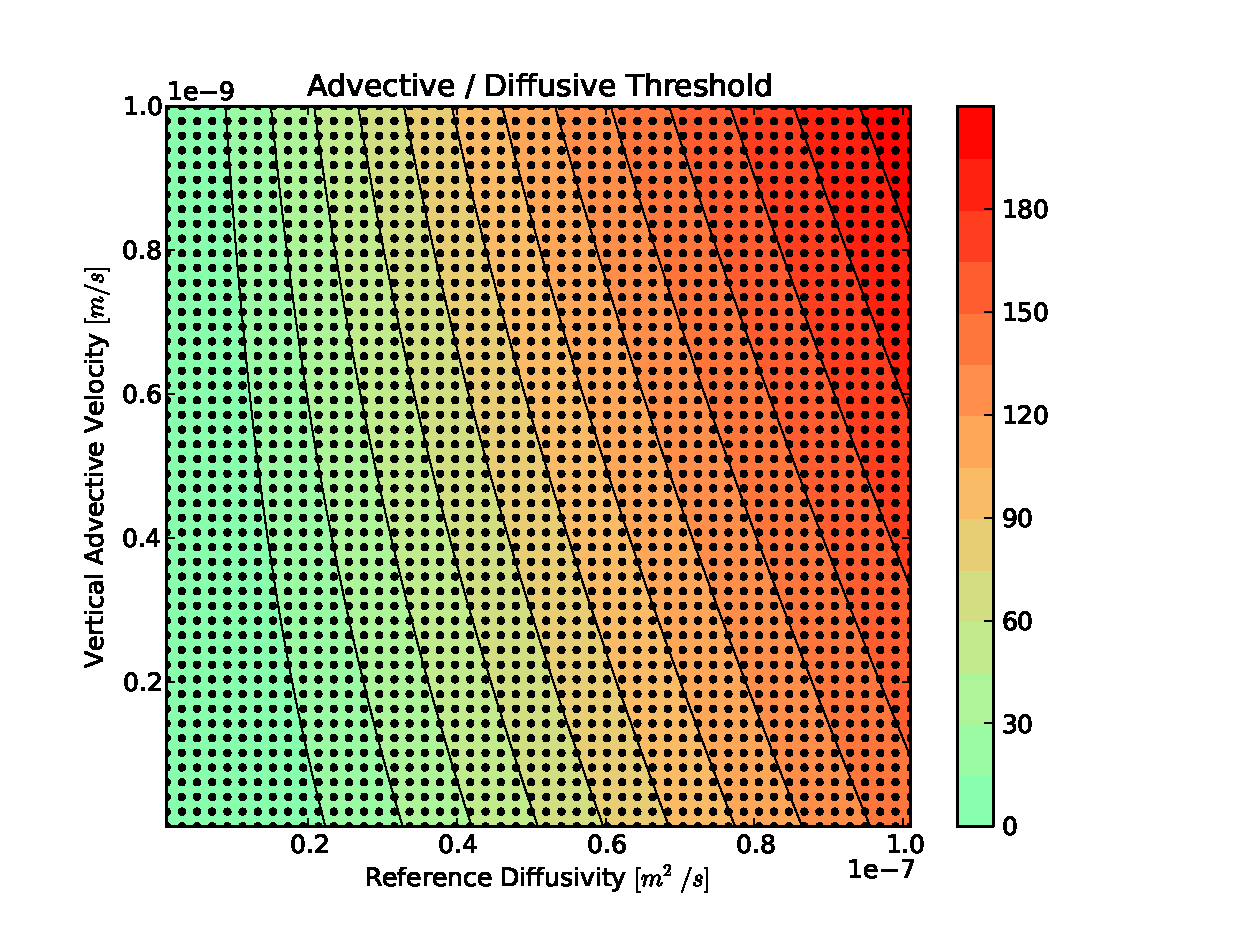
\includegraphics[width=\linewidth]{./chapters/demonstration/bench/adv_vel_diff.eps}
\caption[Advection vs. Diffusion Sensitivity in Cyder]{Dual advective velocity 
and reference diffusivity sensitivity for a non-sorbing, infinitely soluble 
nuclide.}
\label{fig:dr_adv_diff}
\end{figure}
